\Chapter{Folyamat példák}

%https://xflower.hu/blog/az-uzleti-folyamatokrol-bovebben-iii-hogyan-hatarozzam-meg-folyamataimat
%Fenti forrásból gyűjteni adatokat, illetve 

Dolgozatom utolsó tartalmi fejezetének alapjául a 2. fejezethez hasonlóan a(z) \cite{xflower} hivatkozásban megjelölt oldalt használtam alapul, viszont most már csak egy, erre a témára vonatkozó blogbejegytést\cite{xflowutolso} dolgoztam fel és bővítettem saját leírásokkal.
%Ez most még nem igaz

\Section{Áttekintés}

Ez a fejezet bemutatja néhány példa segítségével, hogy hogyan és milyen folyamatokat lehet a program elkészülte után annak használatával modellezni.

\Section{Első példa}

Először nézzünk egy, már létező példát arra, hogy hogyan is néz ki egy olyan folyamatábra, amely egy üzleti folyamatot modellez. Ehhez tekintsük az alábbi \textit{BPMN} (Business Process Model and Notation) diagramot (\ref{fig:bpmn} ábra).

\begin{figure}[h]
\centering
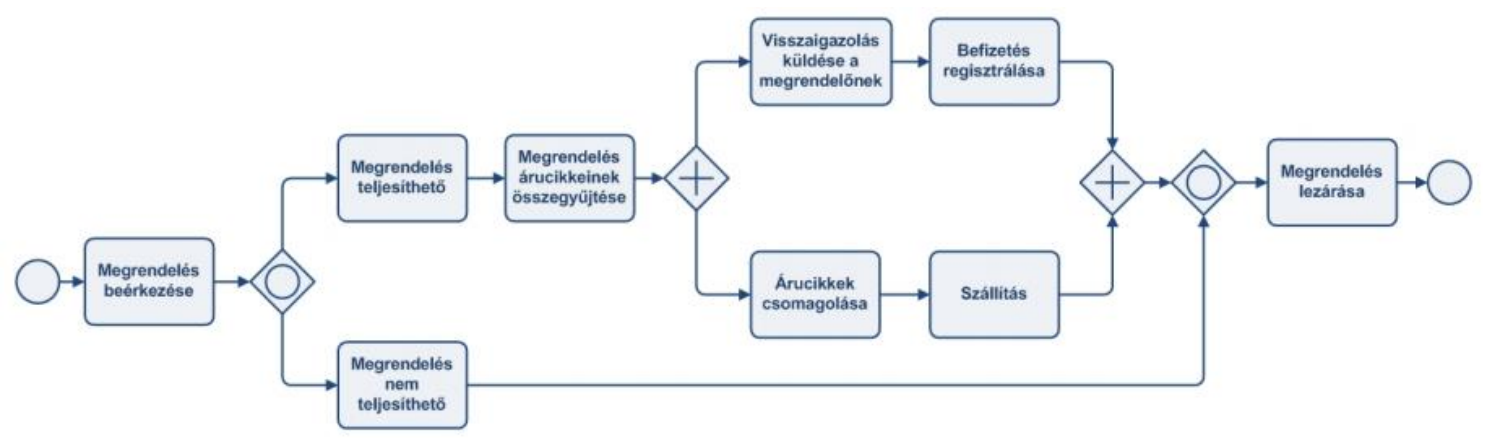
\includegraphics[scale=0.38]{images/BPMN.png}
\caption{BPMN diagram (forrás: \cite{bpmn})}
\label{fig:bpmn}
\end{figure}

Az ábra egy kiváló példa teljes folyamatábrára: Van egy-egy kezdő- és végállapota, minden csomópontba el lehet jutni, és bármelyik csomópontból a végállapotba mehetünk a vonalak és a csomópontok mentén.

A folyamatábrán egy megrendelési folyamatot láthatunk. Első lépésben az adott vállalathoz beérkezik az általuk megrendelt áru. Itt máris útelágazáshoz érkezünk: ha a megrendelés nem teljesíthető valamilyen oknál fogva (például aktuálisan nincs rá kapacitása a cégnek vagy nincs jelen az a személy, aki a megrendeléseket kezeli), akkor máris lezárásra kerül, és végallpotba jutunk a folyamatábrán. Ha viszont minden feltétel adott a megrendeléshez, akkor az teljesíthető. Ekkor összegyűjtik a megrendelés árucikkeit. Ezt követően egy újabb átjáró (vagy elágazás) következik. Láthatjuk, hogy az eddigi két rombusz elem más-más jelölést tartalmaz. Az előbbi egy eldöntendő (igaz vagy hamis) csomópont volt, utóbbi után pedig párhuzamos feladatvégrehajtás következik. Egyfelől az összegyűjtött árucikkeket becsomagolják, majd ezt követően elszállítják a megrendelés helyére, ezzel egyidejűleg pedig értesítik a megrendelőt egy visszaigazolással, és regisztrálják a befizetést. Két újabb rombusz alakzat zárja az azonos jellel megjelölt korábbi útválasztó csomópontokat, és végül lezárásra kerül a megrendelés. Az egész folyamat pedig egy kezdő- és egy végállapot közé van fogva.

A fenti ábra után tekintsük meg, hogy pontosan ugyanez a folyamat hogyan modellezhető a szakdolgozat programjának segítségével.

\begin{figure}[h]
\centering
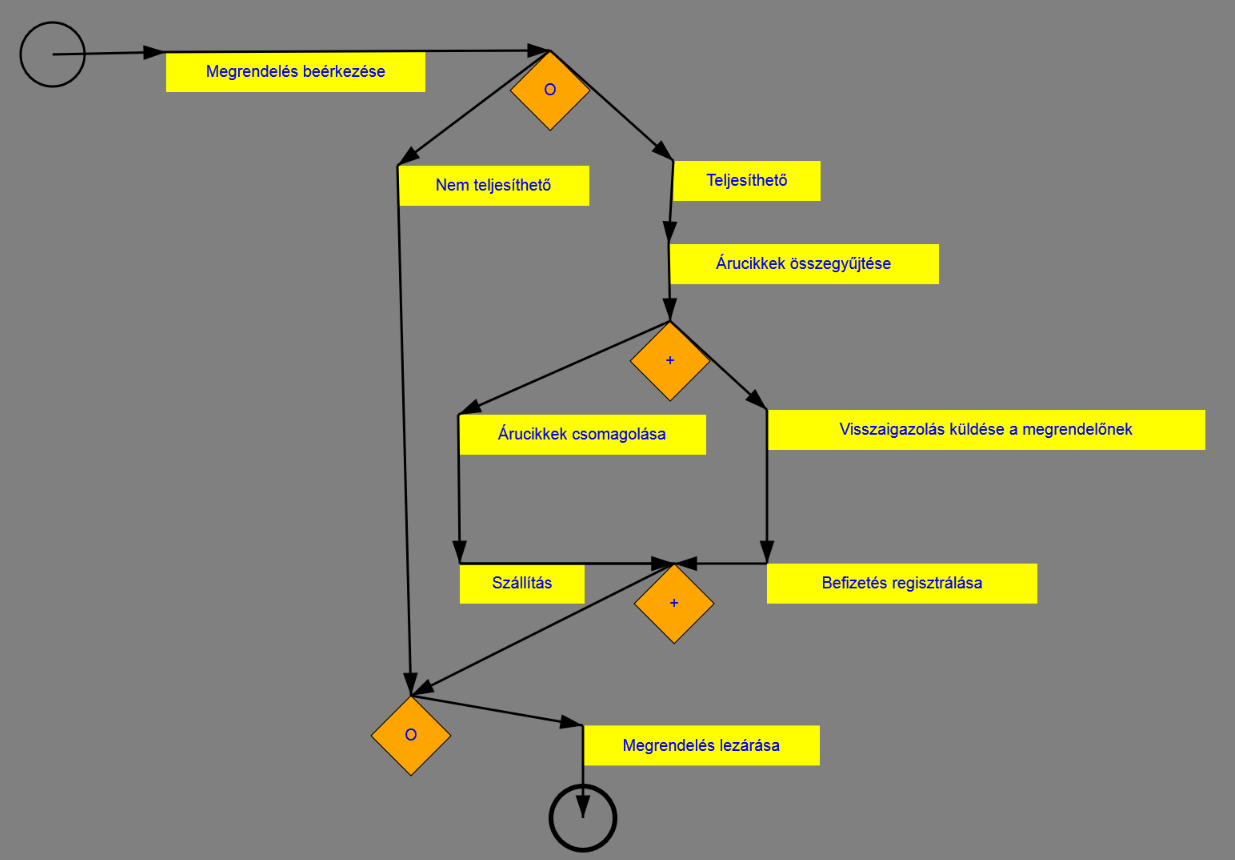
\includegraphics[scale=0.45]{images/pelda1NEMVEGLEGES.png}
\caption{BPMN diagram a saját programmal készítve}
\label{fig:bpmn}
\end{figure}

Némi eltérés felfedezhető a két ábra között. A szakdolgozat alkalmazás színes csomópontokat használ, ami látványosabbá teszi a modellezést, azonban azok összekötésére kisebb hangsúlyt fektet. Előbbi ábrán a csomópontok szövegei több sorba való tagolással vannak megvalósítva, így minden tevékenységet jelölő csomópont azonos méretű. Hosszabb szövegek esetén viszont már nem lesz meg ez az egység. A szakdolgozat programjában ellenben minden csomópont pontosan azonos méretűre hozható a benne lévő szöveg hosszától függetlenül.

\Section{Második példa}

Második példaként hozzunk létre egy létező mintától függetlenül egy folyamatábrát.


